%
% Documento: Fundamentação Teorica
%

%\vspace{3cm}%Espaçamento entre linhas

\chapter{\textbf{DESCRIÇÃO DA SOLUÇÃO}}\label{chap:descSolucao}

Visando atender o objetivo deste trabalho de desenvolver um sistema capaz de gerenciar animais, uma solução web foi implementada. Este capítulo detalha o desenvolvimento dessa solução, partindo do modelo de requisitos do mesmo.

A análise de requisitos do presente trabalho foi realizada através de conversas com os pecuáristas do estudo de caso. Para delimitar as funcionalidades foi elaborado um diagrama de casos de uso contendo as mesmas.

\section{MODELO DE REQUISITOS}

Para a modelagem de requisitos, utilizou-se o diagrama de casos de uso porque, "ele possibilita a compreensão do comportamento externo do sistema, tornando possível ter uma visão das funcionalidades do sistema" \cite{guedes18}. Neste sentido o diagrama a seguir mostra um usuário desempenhando as funções representadas pelos casos de uso.

\begin{figure}[H]
	\begin{center}
		\caption{Diagrama de Casos de Uso do sistema}
		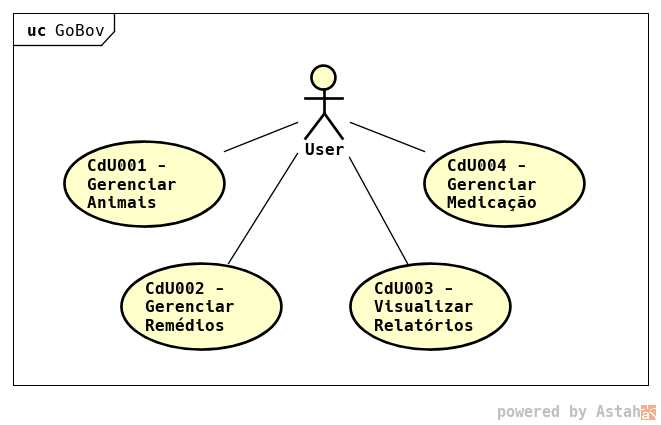
\includegraphics[width=\textwidth]{../img/casosdeuso.png}

		Fonte: Autoria própria.
	\end{center}
	\label{CdU}
\end{figure}

O caso de uso (CdU) Gerenciar Animal trata das operações realizadas com os animais, no caso, criar um animal, ler as informações dele, atualizar suas informações e deleta-lo. Os casos de uso Gerenciar Remédios e Gerenciar Medicações se referem as mesmas operações, porém, com seus respectivos objetos. O caso de uso Visualizar Relatórios se refere a visualização das informações disponibilizadas pelo sistema, como os gráficos de pesos de animais, aqui chamados de relatórios.


\subsection{\textbf{Telas do Sistema}}\label{telas}
Nesta subseção serão apresentadas as telas do sistema, quais informações elas aoresentam e quais ações elas possibilitam.

\begin{itemize}
\item IV001

A figura 5 é a tela de login do sistema. Nela, o usuário pode se autenticar ou ser direcionado para outra página com o propósito se registrar.
\begin{figure}[H]
	\begin{center}
		\caption{Login no sistema}
		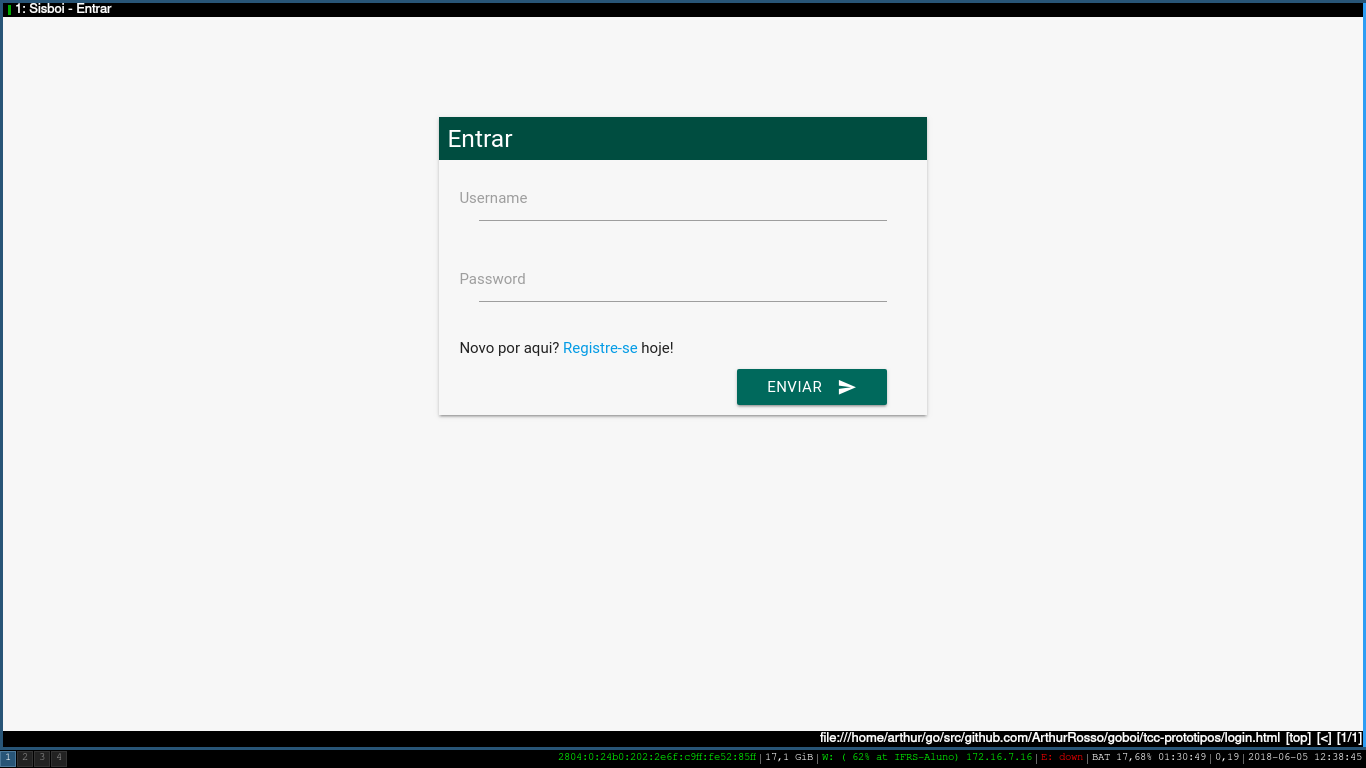
\includegraphics[width=\textwidth]{../img/prototipos/login.png}

		Fonte: Autoria própria.
	\end{center}
\end{figure}

\item IV002

A figura 6 é a tela inicial do sistema. Nela aparecem informações sobre a propriedade, como a quantidade total de animais, remédios e medicações. O usuário também pode ir para a tela de lista de animais, lista de Remédios, ou lista de medicações, ou ser direcionado para o menu, com as preferencias do usuário, nela é possível criar e deletar propósitos, tipos e raças de animais, além dos tipos de remédios.

\begin{figure}[H]
	\begin{center}
		\caption{Página inicial do sistema}
		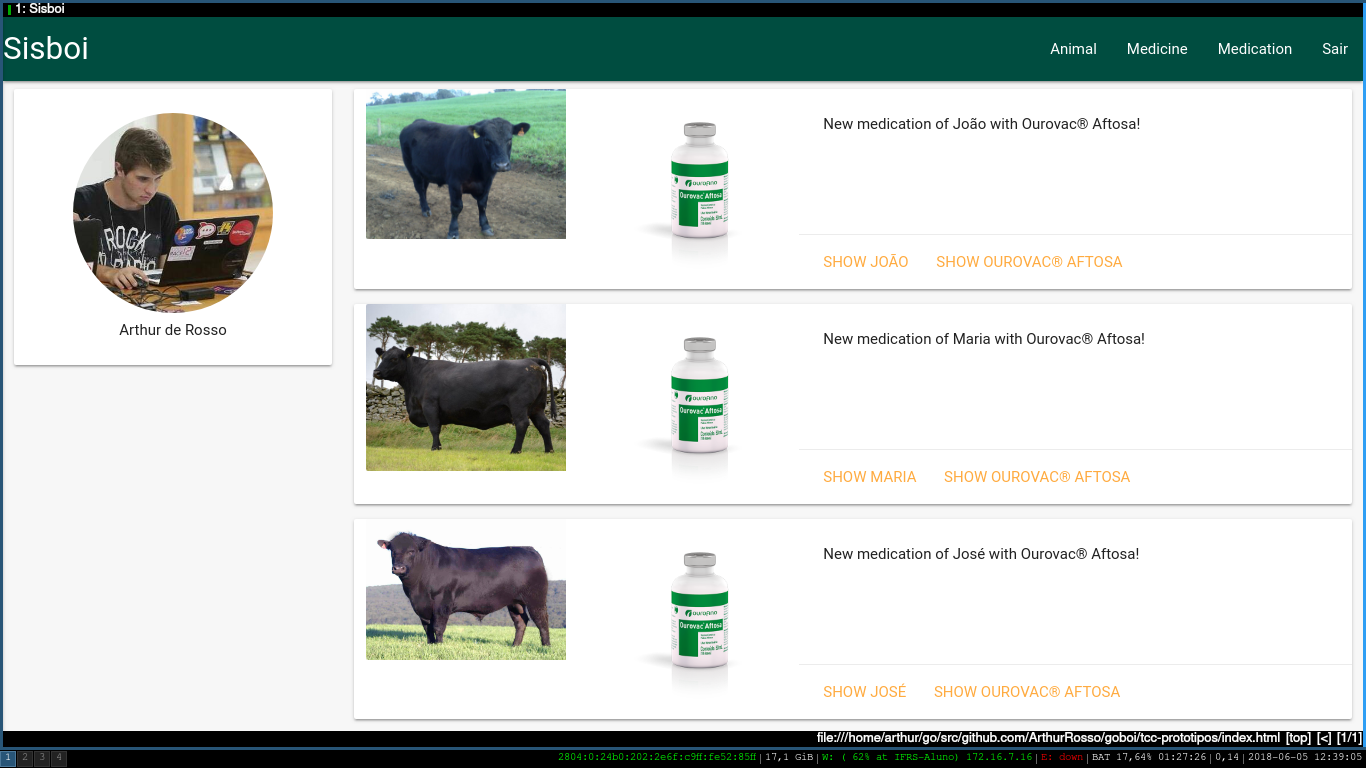
\includegraphics[width=\textwidth]{../img/prototipos/index.png}

		Fonte: Autoria própria.
	\end{center}
\end{figure}

\item IV003

A figura 7 é a página de lista de animais é apresentada a lista de animais com alguns atributos e 3 ícones, um para deletar o animal, outro para registrar uma medicação e outro para registrar um peso. É mostrada uma barra de consulta, para filtrar os resultados. O usuário pode adicionar um animal, adicionar uma medicação a um animal, pesar um animal, deletar um animal ou ir para a tela de perfil do animal.
\begin{figure}[H]
	\begin{center}
		\caption{Página do animais}
		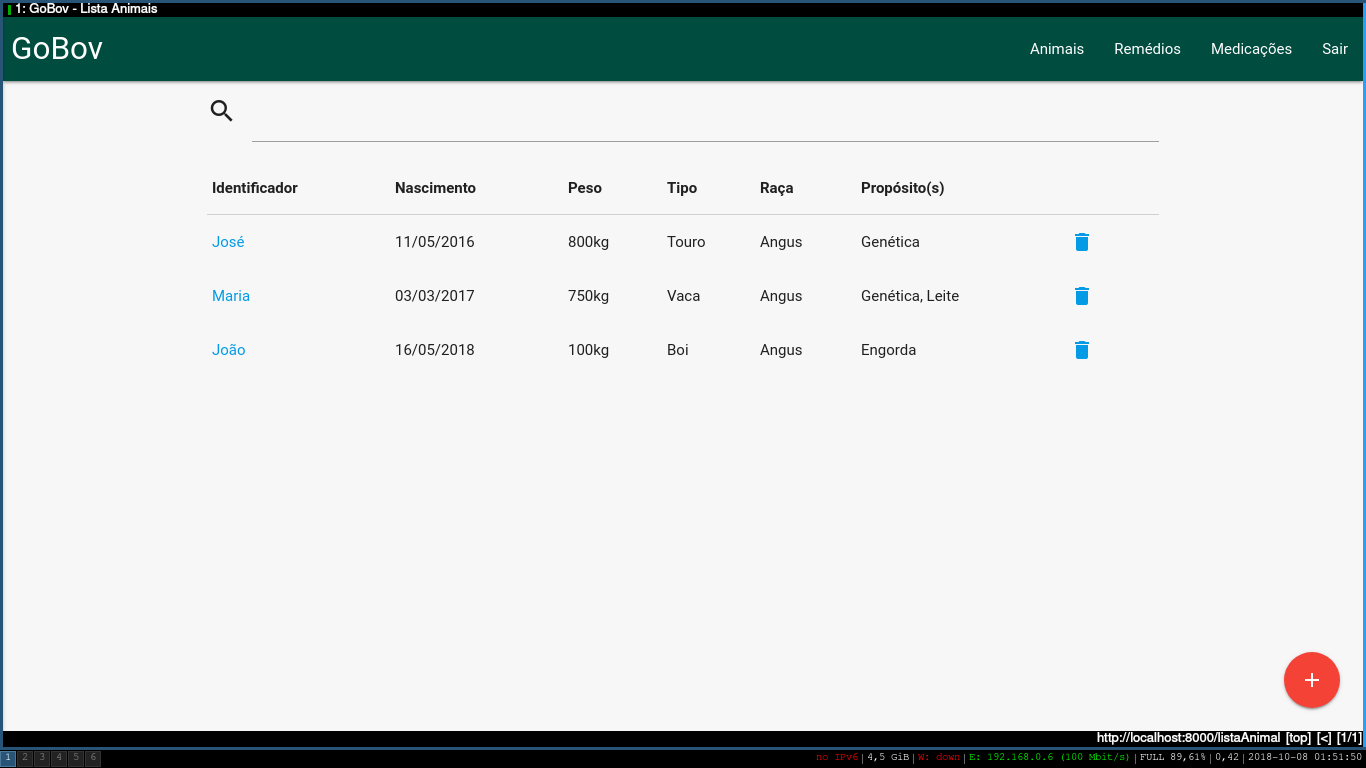
\includegraphics[width=\textwidth]{../img/prototipos/listaAnimal.png}

		Fonte: Autoria própria.
	\end{center}
\end{figure}

\item IV004

A figura 8 é a página de adicionar animal. O usuário insere as informações do animal e solicita salvar, após isso ele é direcionado para a página de perfil do animal recém adicionado.
\begin{figure}[H]
	\begin{center}
		\caption{Página de adicionar animal}
		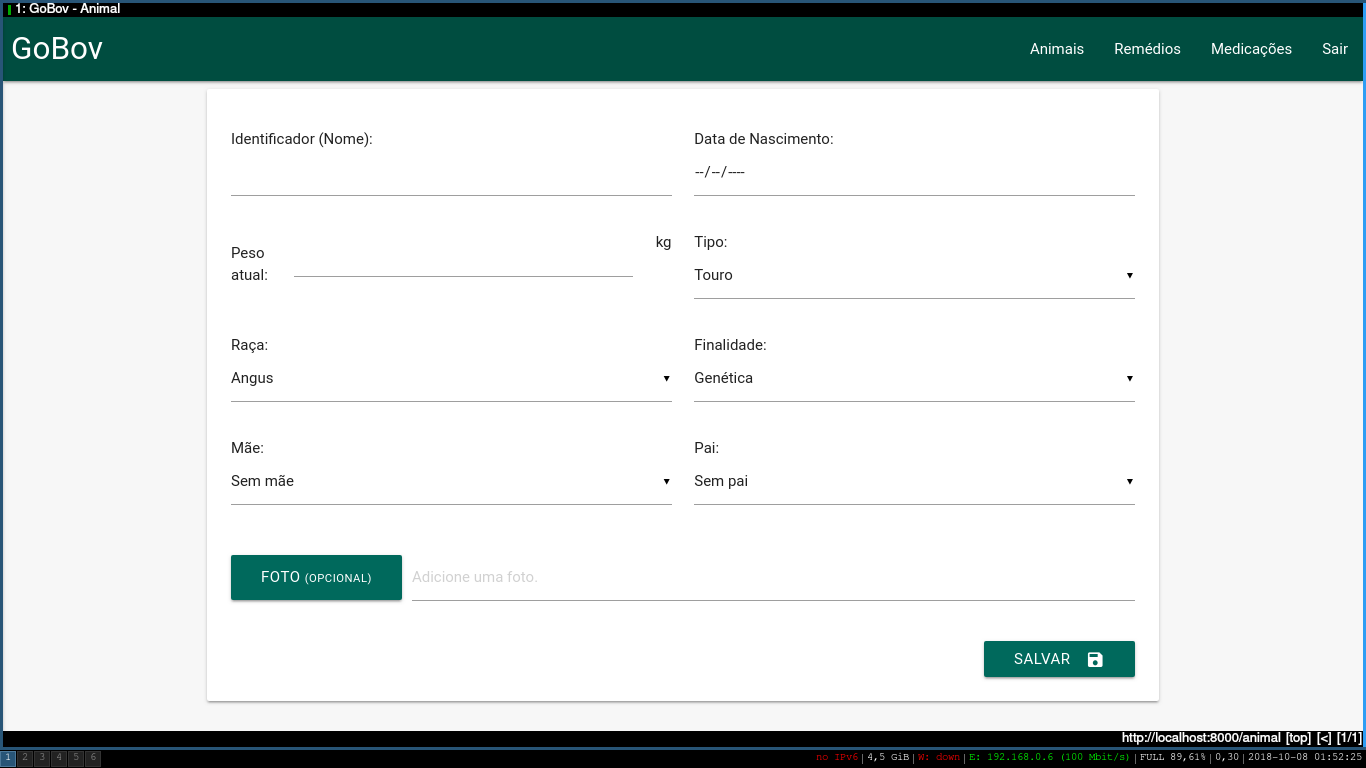
\includegraphics[width=\textwidth]{../img/prototipos/addAnimal.png}

		Fonte: Autoria própria.
	\end{center}
\end{figure}


\item IV005

A figura 9 é a página de lista de remédios, é mostrado as informações dos remédios do usuário. Na página o usuário pode adicionar, deletar ou editar um remédio.
\begin{figure}[H]
	\begin{center}
		\caption{Página de remédios}
		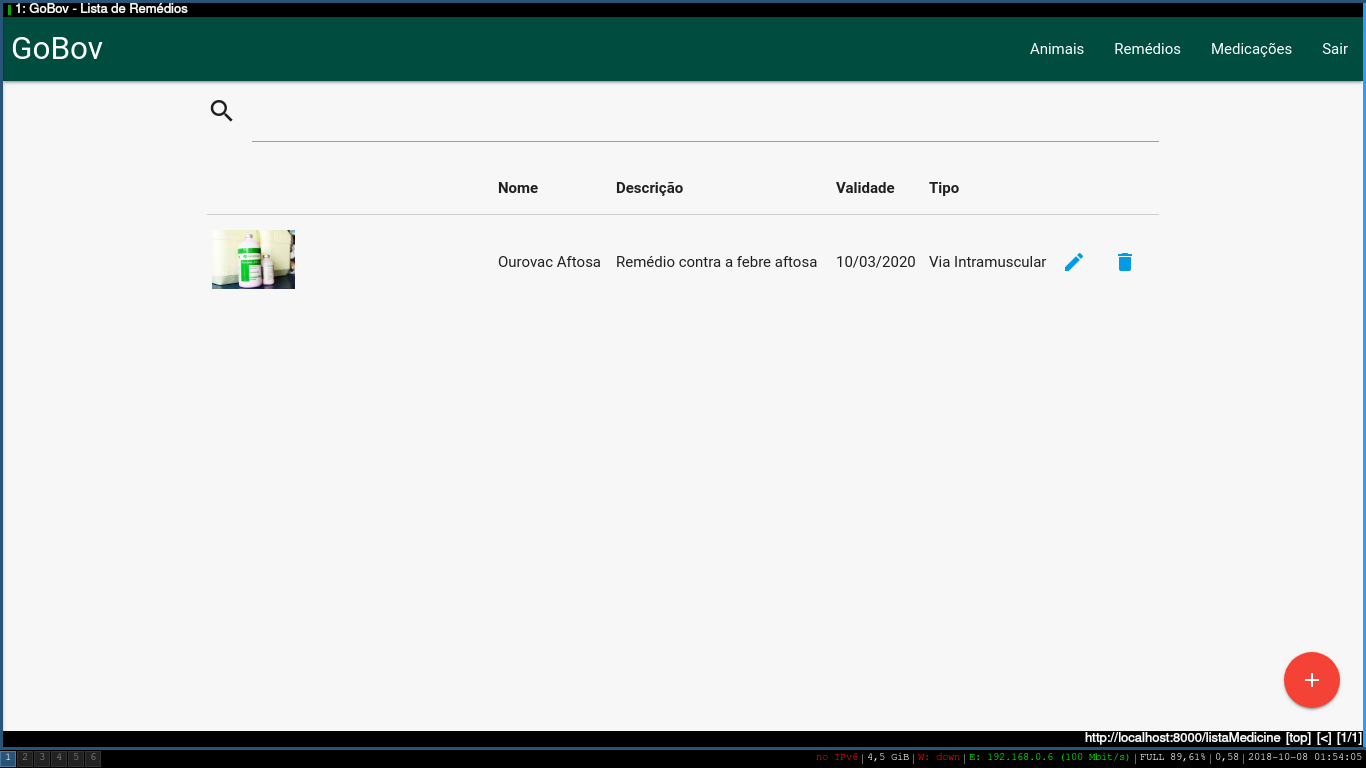
\includegraphics[width=\textwidth]{../img/prototipos/listaRemedio.png}

		Fonte: Autoria própria.
	\end{center}
\end{figure}

\item IV006

A figura 10 é a página de adicionar remédio. O usuário insere as informações do remédio e solicita salvar, após isso ele é direcionado para a página da lista de remédios.
\begin{figure}[H]
	\begin{center}
		\caption{Página de adicionar remédio}
		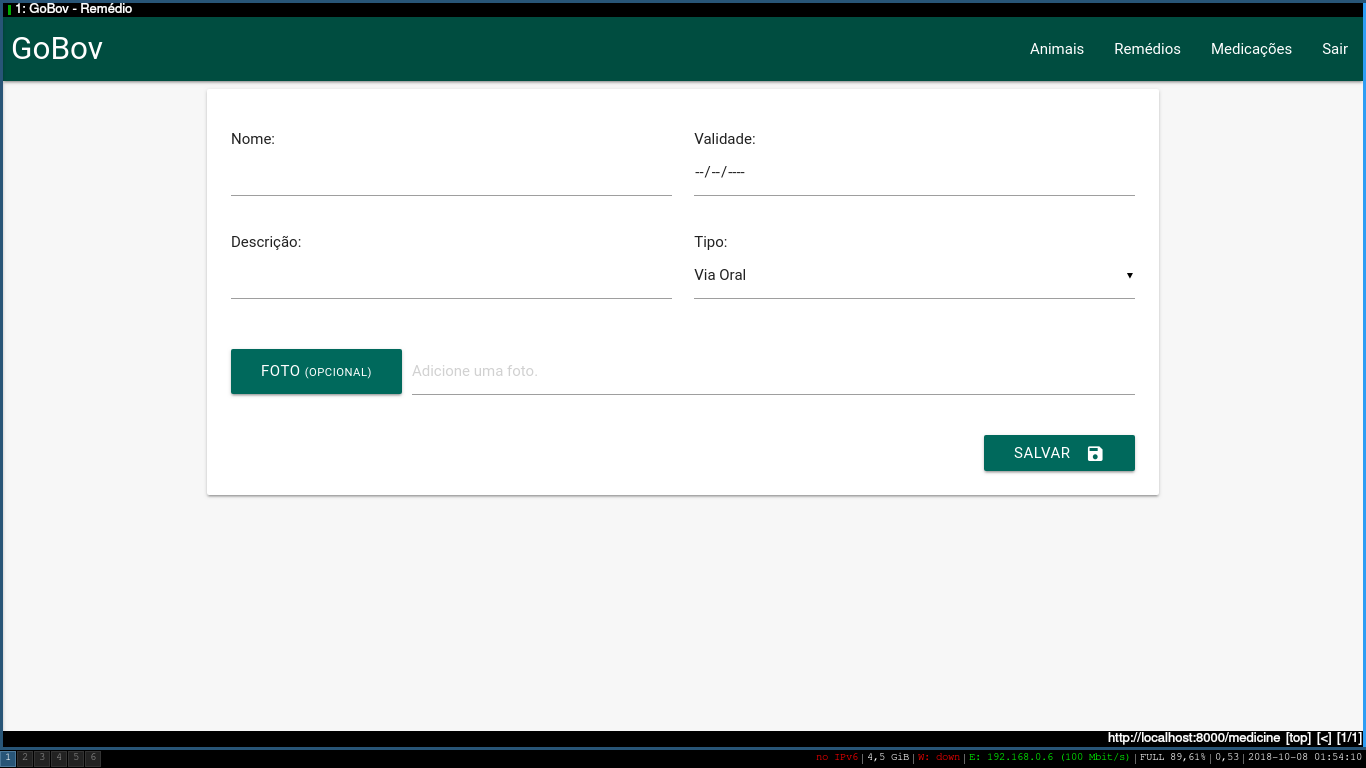
\includegraphics[width=\textwidth]{../img/prototipos/addRemedio.png}

		Fonte: Autoria própria.
	\end{center}
\end{figure}


\item IV007

A figura 11 é a página de lista de medicações, é apresentado as medicações realizadas com uma descrição, a data da realização, a lista de animais medicados e os remédios utilizados. Nela, o usuário pode adicionar ou deletar uma medicação.
\begin{figure}[H]
	\begin{center}
		\caption{Página de medicações}
		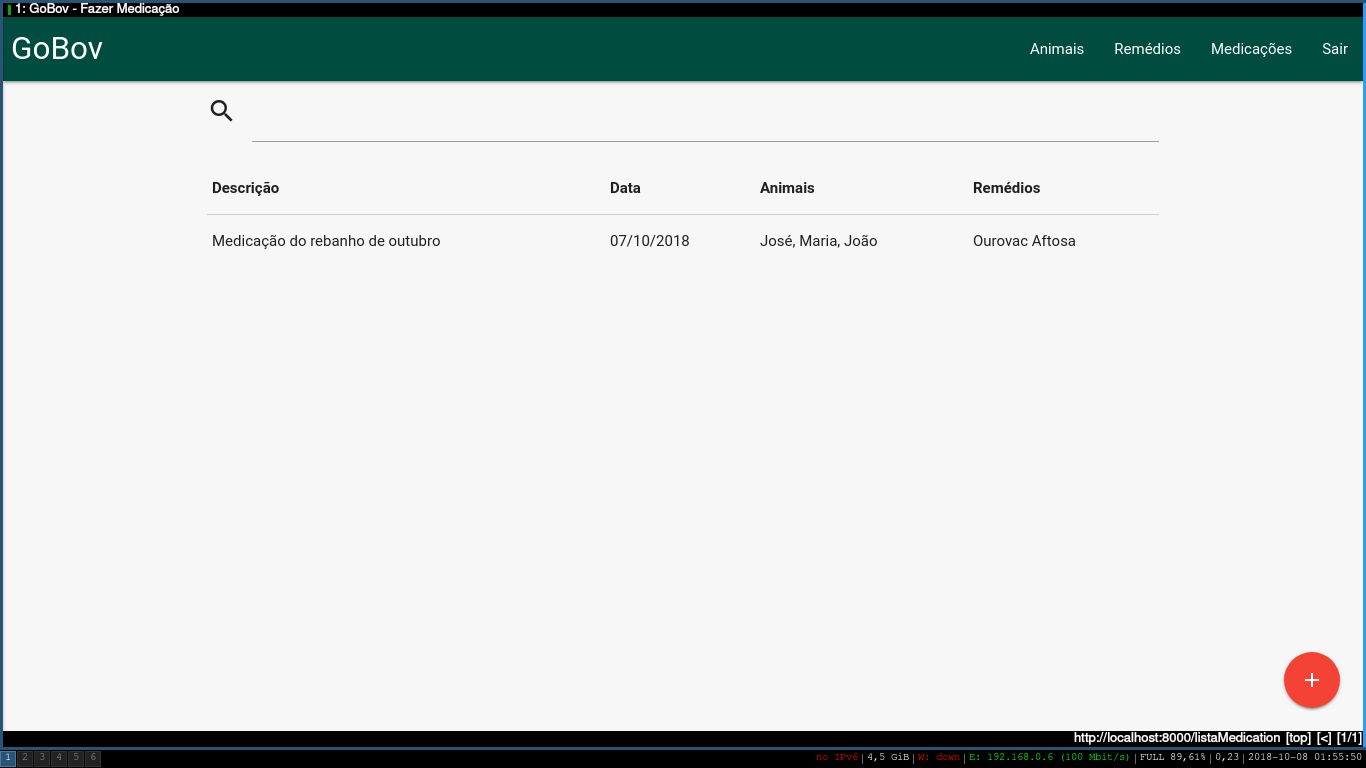
\includegraphics[width=\textwidth]{../img/prototipos/listaMedicacao.png}

		Fonte: Autoria própria.
	\end{center}
\end{figure}

\item IV008

A figura 12 é a página de adicionar medicação. Nela o usuário insere uma descrição, a data que a medicação ocorreu, os animais medicados e os remédios utilizados.
\begin{figure}[H]
	\begin{center}
		\caption{Página de adicionar medicação}
		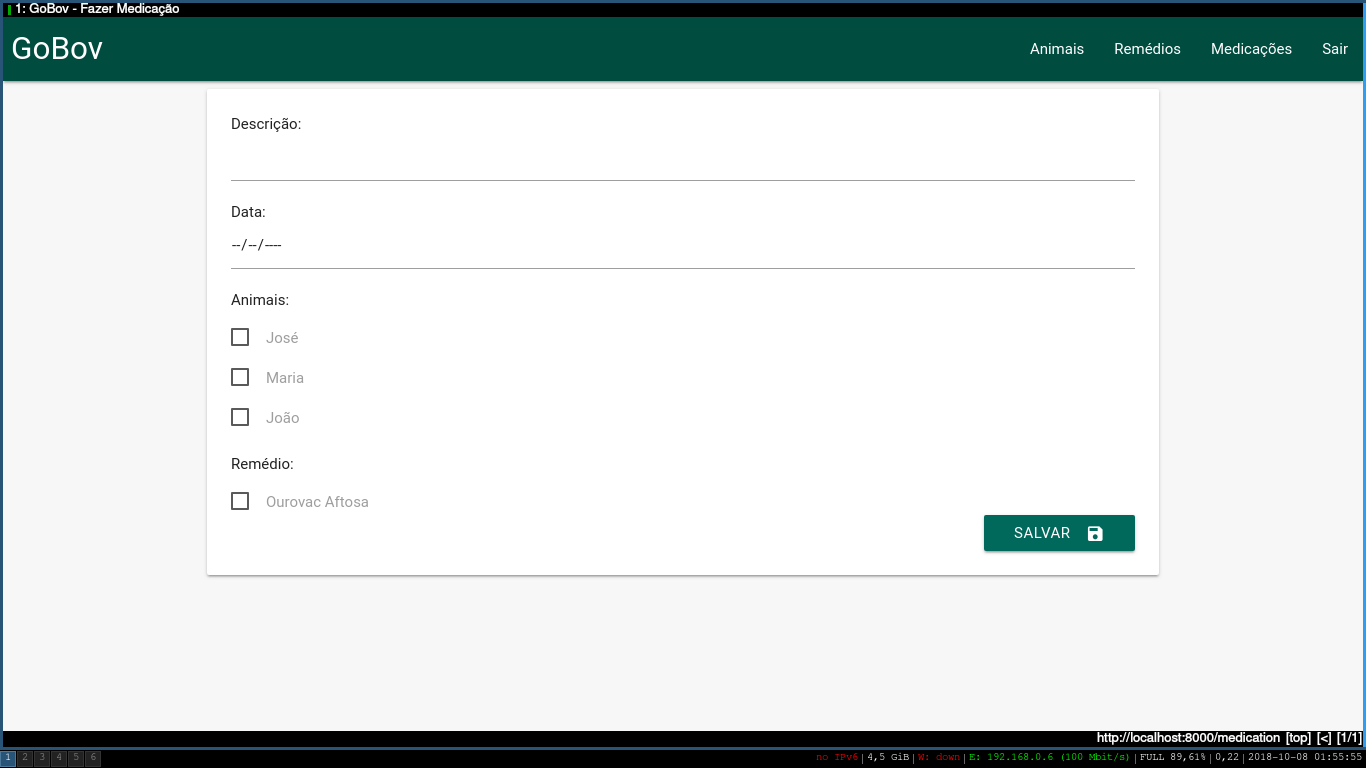
\includegraphics[width=\textwidth]{../img/prototipos/addMedicacao.png}

		Fonte: Autoria própria.
	\end{center}
\end{figure}

\item IV009

A figura 13 é a página de perfil do animal. Nela, são apresentadas todas as informações do animal, inclusive um histórico do que aconteceu com o animal. O usuário pode editar, consultar detalhes, gerenciar uma pesagem do animal ou consultar relatórios individuais do animal.
\begin{figure}[H]
	\begin{center}
		\caption{Página de perfil do animal}
		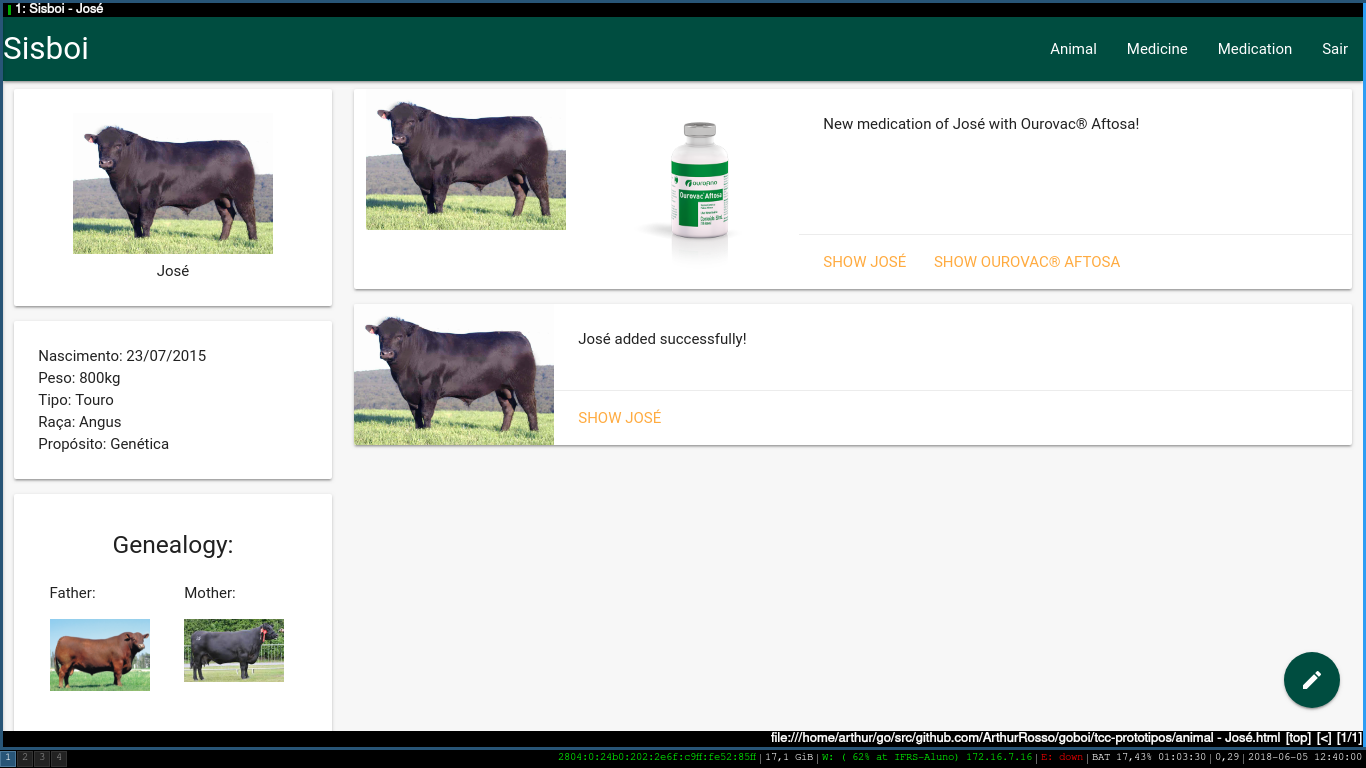
\includegraphics[width=\textwidth]{../img/prototipos/perfil.png}

		Fonte: Autoria própria.
	\end{center}
\end{figure}


\item IV010

A figura 14 é a página de edição do animal. Nela o usuário pode editar as informações básicas do animal.
\begin{figure}[]
	\begin{center}
		\caption{Página de edição do animal}
		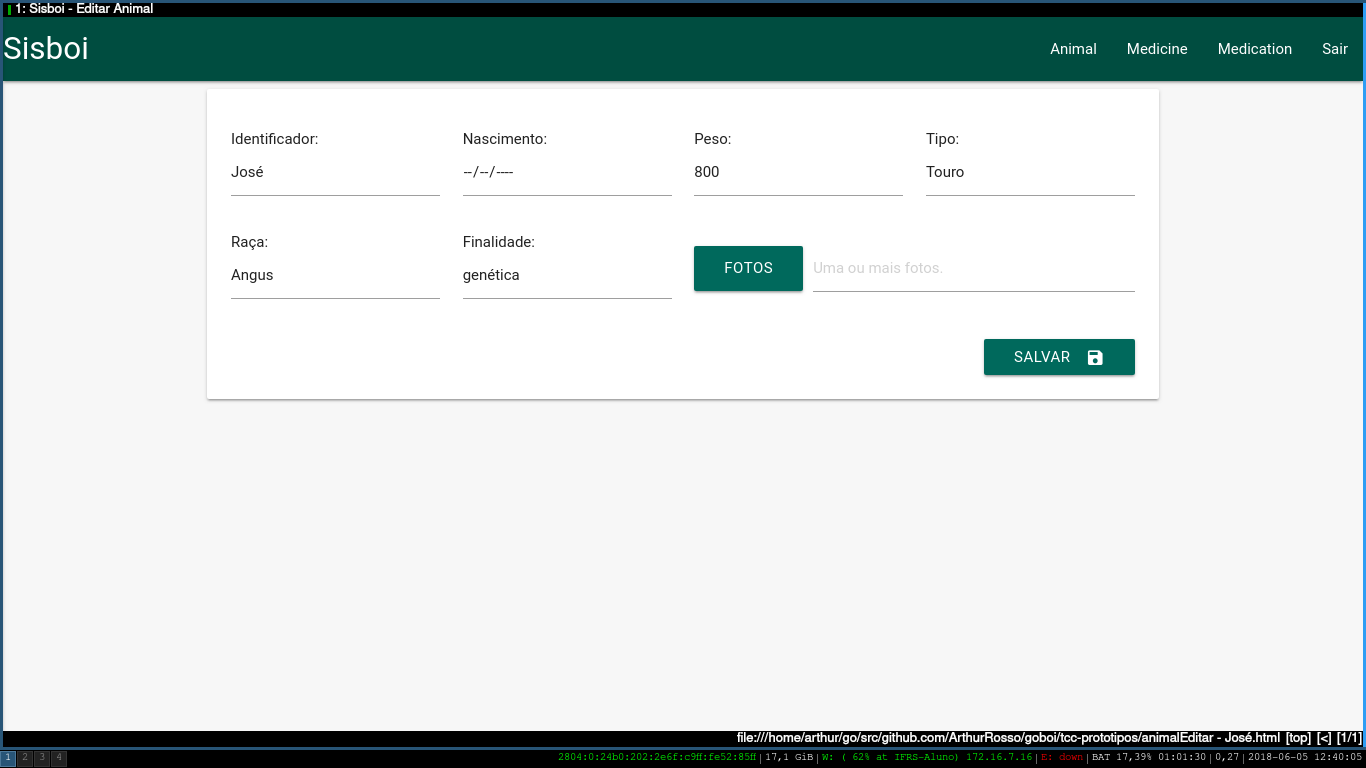
\includegraphics[width=\textwidth]{../img/prototipos/editar.png}

		Fonte: Autoria própria.
	\end{center}
\end{figure}

\newpage
\item IV011

A figura 15 é a página de pesagem. É apresentada a lista de pesagens do animal e o usuário pode gerenciar o peso de um animal.
\begin{figure}[H]
	\begin{center}
		\caption{Página de pesagem do animal}
		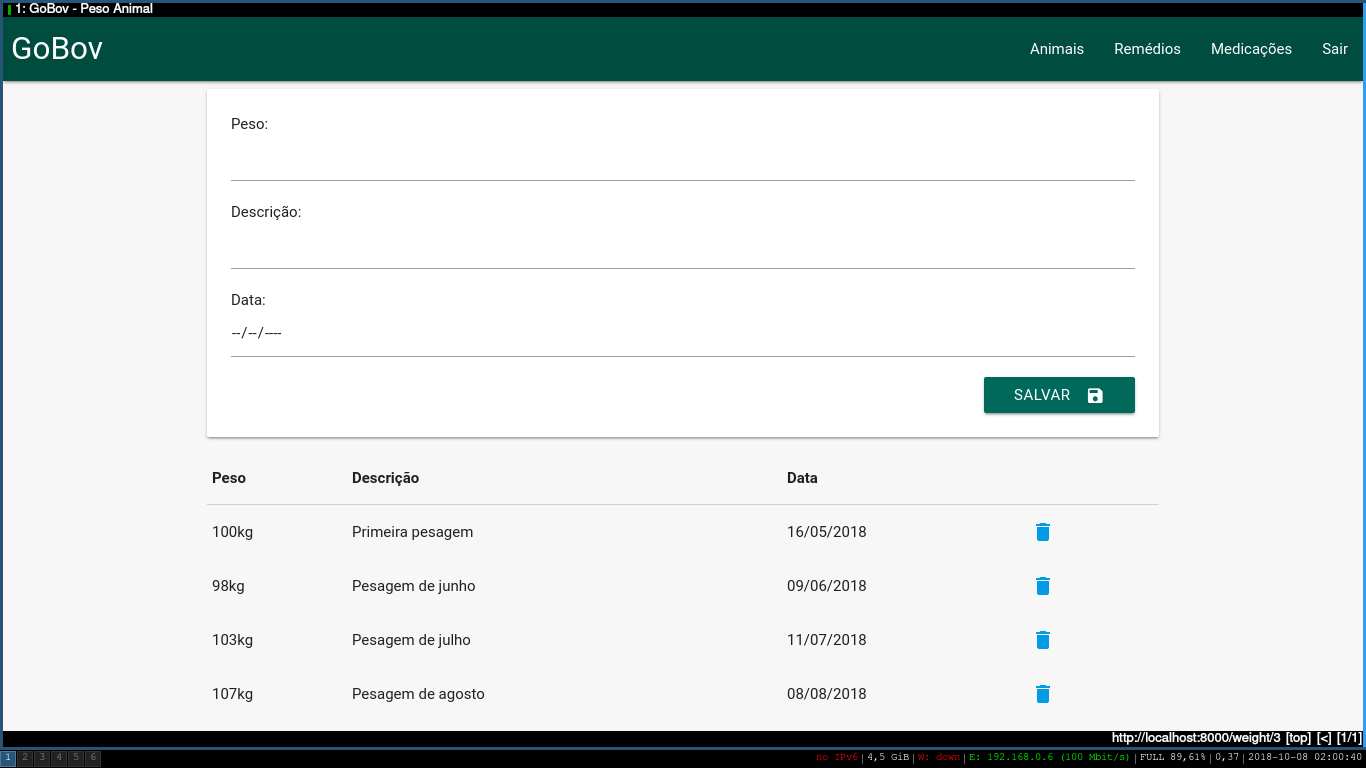
\includegraphics[width=\textwidth]{../img/prototipos/addPeso.png}

		Fonte: Autoria própria.
	\end{center}
\end{figure}

\item IV012

A figura 16 é a página de relatórios individuais do animal a qual é apresentado o gráfico do peso do animal ao longo do tempo.
\begin{figure}[H]
	\begin{center}
		\caption{Página de pesagem do animal}
		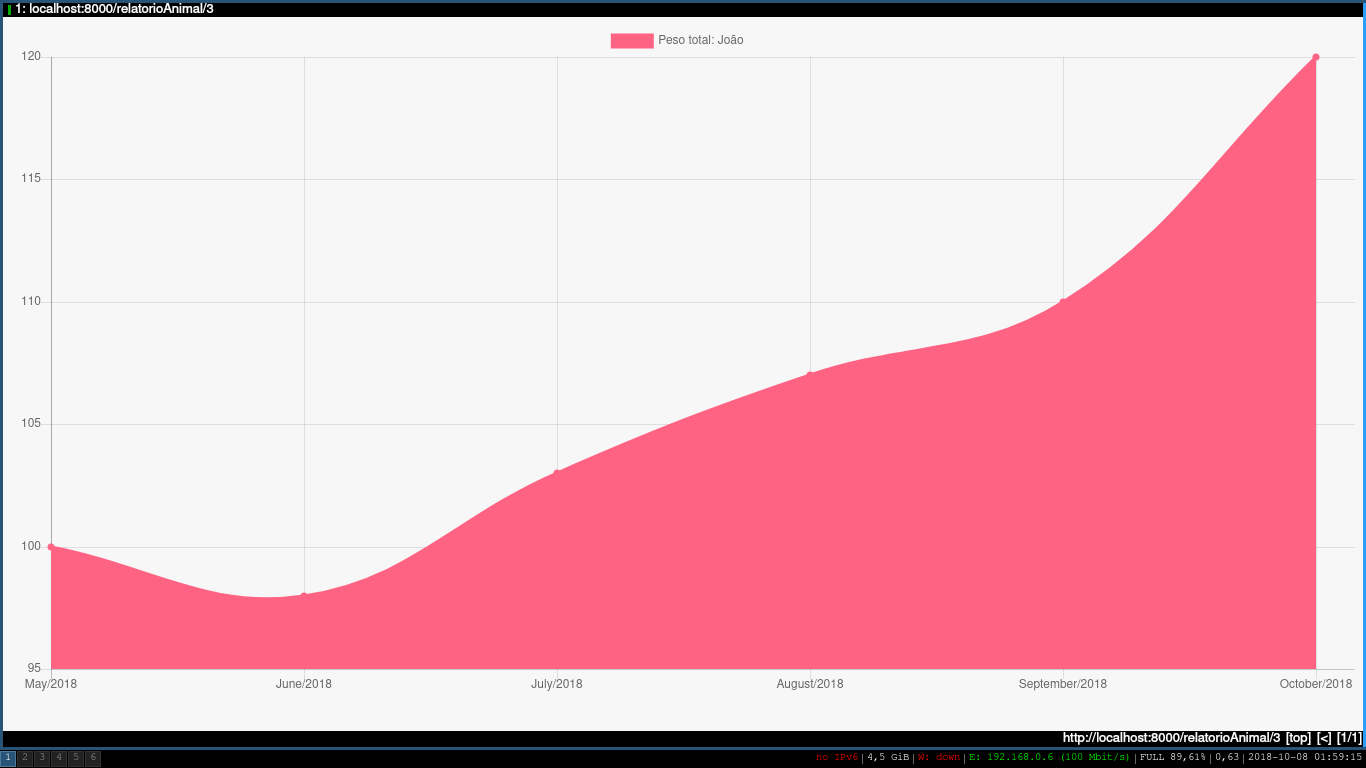
\includegraphics[width=\textwidth]{../img/prototipos/relatorio.png}

		Fonte: Autoria própria.
	\end{center}
\end{figure}

\end{itemize}

\section{MODELO ENTIDADE RELACIONAMENTO}

O diagrama a seguir mostra o modelo Entidade Relacionamento (ER), que caracteriza a abstração do banco de dados representando a relação do animal com o usuário, com a foto, com o peso, com o propósito, com a raça, com o tipo, e com a remédio, na qual é chamada de medicação. Por sua vez, o remédio também tem uma relação além da medicação, que é o tipo.

\begin{figure}[H]
	\begin{center}
		\caption{Modelo ER}
		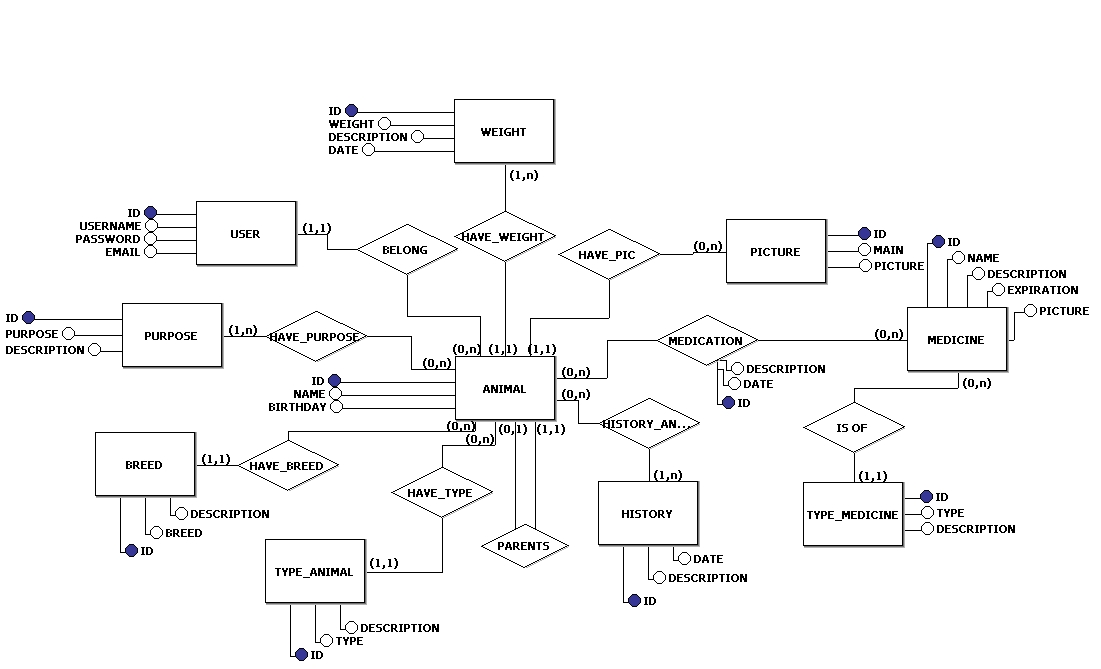
\includegraphics[width=\textwidth]{../img/erdoboi.jpg}

		Fonte: Autoria própria.
	\end{center}
	\label{er}
\end{figure}
